\documentclass[11pt,a4paper]{article}
\usepackage{bbm,amsthm,amsfonts,amssymb,amsmath,latexsym,epic,eepic}
\usepackage{marvosym,graphicx,fancyhdr,bbm}
\usepackage{graphicx}
\usepackage{color}
\usepackage[rflt]{floatflt}
\usepackage{colortbl}
\definecolor{Grey}{rgb}{0.5,0.5,0.5}
\definecolor{Red}{rgb}{1.0,0.0,0.0}

\usepackage{typearea}
\areaset{156mm}{235mm}
%\setlength{\parskip}{5pt plus 2pt minus 1pt}
\setlength{\parindent}{0pt}

% use \M for matrices and \V for vectors in math mode
\newcommand{\M}[1]{\mathbf{#1}}
\newcommand{\V}[1]{\mathbf{#1}}
\newcommand{\norm}[1]{\left | \left | #1 \right | \right |}
\newcommand{\RR}{\mathbbm{R}}        % set of real numbers


\renewcommand\floatpagefraction{0.8}
\renewcommand\topfraction{1}
\renewcommand\bottomfraction{0.9}
\renewcommand\textfraction{0.0}
%\def\dbltopfraction{1.0}
%\def\bottomfraction{1.0}
%\def\dblfloatpagefraction{0.8}


\makeatletter
\renewenvironment{thebibliography}[1]
     {\section*{\refname}%
      \@mkboth{\MakeUppercase\refname}{\MakeUppercase\refname}%
	 \parsep0mm
	 \itemsep0mm
	 %\labelsep0mm
	 %\itemindent0mm
      \list{\@biblabel{\@arabic\c@enumiv}}%
           {\settowidth\labelwidth{\@biblabel{#1}}%
            \leftmargin\labelwidth
            \advance\leftmargin\labelsep
            \@openbib@code
            \usecounter{enumiv}%
            \let\p@enumiv\@empty
            \renewcommand\theenumiv{\@arabic\c@enumiv}}%
      \sloppy
      \clubpenalty4000
      \@clubpenalty \clubpenalty
      \widowpenalty4000%
      \sfcode`\.\@m}
     {\def\@noitemerr
       {\@latex@warning{Empty `thebibliography' environment}}%
      \endlist}
\renewcommand\newblock{\hskip .11em\@plus.33em\@minus.07em}
\let\@openbib@code\@empty
\makeatother



\begin{document}\sloppy

\title{\Large\bf Vergleich der Pfadverfolgung mit Odometrie und AMCL \footnotetext{Diese Arbeit ist Bestandteil des Praktikums zur Mess- und Regelungstechnik}}

\author{Kai Hofmann und Barbara Fischbach\\
  Robotik und Telematik \\
  Universit\"at W\"urzburg\\
  Am Hubland, D-97074 W\"urzburg\\
{\small \texttt{barbara.fischbach@uni-wuerzburg.de}}\\
{\small \texttt{kai.hofmann@uni-wuerzburg.de}}}

\date{}




\maketitle

\newpage

\tableofcontents{}

\newpage

\twocolumn

\section*{Abstract}
\addcontentsline{toc}{section}{Abstract}
{
\textbf{Die autononome Fortbewegung von Fahrzeugen spielt heutzutage immer eine gr\"o\ss{}ere Rolle. Dazu werden verschiedene Algorithmen, zur Lokalisierung, Kartierung, und Pfadverfolgung genutzt. Diese wurden auf einem realen Roboter implementiert und getestet. Nicht nur im Weltall, wo wir unbedingt darauf angewiesen sind, dass Systeme autonom funktionieren, sondern auch auf der Erde, um Systeme sicherer und bequemer f\"ur den Benutzer zu machen. }


\section{Einleitung}
Um das überaus komplexe Thema verst\"andlicher zu machen und Algorithmen vorstellbar zu erkl\"aren, wird im folgenden ein Fraunhofer-Roboter benutzt, der anhand Odometrie,... sich selbst\"andig in einem bekannten Raum zurechtfinden kann.

\section{ROS}
Für die Implementierung und Tests der Algorithmen wird das \textit{Robot Operating System}, kurz ROS genutzt. Es ist kein Betriebssystem im eigentlichen Sinn, sondern ein Framework. Es ermöglicht Hardware-Abstraktion, Paket-Managment und stellt eine Middleware bereit mit der verschiedene Prozesse kommunizieren können. \cite{rosWiki}
 

\section{Lokalisation}
\subsection{Odometrie}
{Die Odometrie beruht auf einer relativen Positionsbestimmung, dabei wird aus der vorher bekannten Position und der zur\"uckgelegten Weg-strecke die neue Position berechnet. Auf kurzen Distanzen liefert die Odometrie sehr genaue Ergebnisse. Mit wachsender Entfernung nehmen auch Fehler durch unterschiedliche Dr\"ucke in den Reifen oder Reibung zu.
	
	}
\subsection{Adaptive  Monte Carlo Localisation}
Im folgenden als AMCL abgek\"urzt, ist ein Algorithmus zur Lokalisation von Robotern. Der Roboter ben\"otigt eine Karte der Umgebung. Auf der Karte sellt er Hypothesen auf, wo er sich auf der Karte befindet und wohin er schaut. Diese Hypothesen kann man sich als virtuelle Roboter vorstellen. Fährt der reale Roboter, so fahren auch die virtuellen Roboter. Dann werden reale Sensormesswerte mit denen der virtuellen Robotern abgelichen. Virtuelle Roboter mit unstimmigen Daten werden gel\"oscht. Der virtuelle Roboter  mit besten den Übereinstimmungen, ist die beste Estimation der Pose. 


\subsection{Odometrie und AMCL im Vergleich}
Um die Lokalisation durch AMCL und Odometrie miteinander zu vergleichen f\"ahrt der Roboter einen "Acht"-f\"ormigen Pfad ab. Die Steuerung erfolgt manuell.  

->insert Diagramm mit Position durch Odometrie und AMCL 


Man erkennt folgende Unterschiede ...


\section{Kartierung mit Gmapping} \cite{gmapping}
F\"ur die Lokalisation (zum Beispiel mit AMCL) eines Roboters ist eine Karte notwendig. Um diese zu erstellen kann der Gmapping Algorithmus verwendet werden. Die Herausforderung liegt dabei in der gleichzeitigen Lokalisierung und Kartierung, dem \textit{simultaneous localization and mapping} Problem kurz SLAM. Denn beide bedingen sich gegenseitig. Um zum Beispiel zwei Laserscans zu einer Karte zusammenzuf\"ugen, m\"ussen die relativen Posen der Aufnahmen bekannt sein. Also ein Lokalisierungsproblem. Und um sich mit dem Laserscanner zu lokalisieren, benötigt man wiederum Kartendaten. 



g von Gmapping erklären!


Bild von der Karte einfügen

Das Untergeschoss des Informatikinstituts ist mit einem Roboter, der mit einem Sick-Laserscanner ausgestattet ist, aufgenommen worden. Um diese Karte korrekt auzunehmen werden nur so und soviel Partikel ben\"otigt. Die Aufnahme ist bis auf einen 1 cm genau und zeigt keine signifikanten Fehler. Bewegte Objekte wie Menschen werden erkannt und nicht in der Karte verzeichnet. Dagegen sorgt helles Licht, das durch die Fensterfronten scheint f\"ur eine Ungenauigkeit und kann nicht als klare Begrenzung festgestellt werden.
(Bild einfügen, in dem man Ungenauigkeit an Fenster sieht!) F\"ur klare Linie wie W\"ande ist es wichtig, das Gel\"ande mit einem Geschwindgkeitslimit von 1 m/s abzufahren. (Eventuell unsere erste Karte mit Dorits vergleichen?)

\begin{figure}[h]
	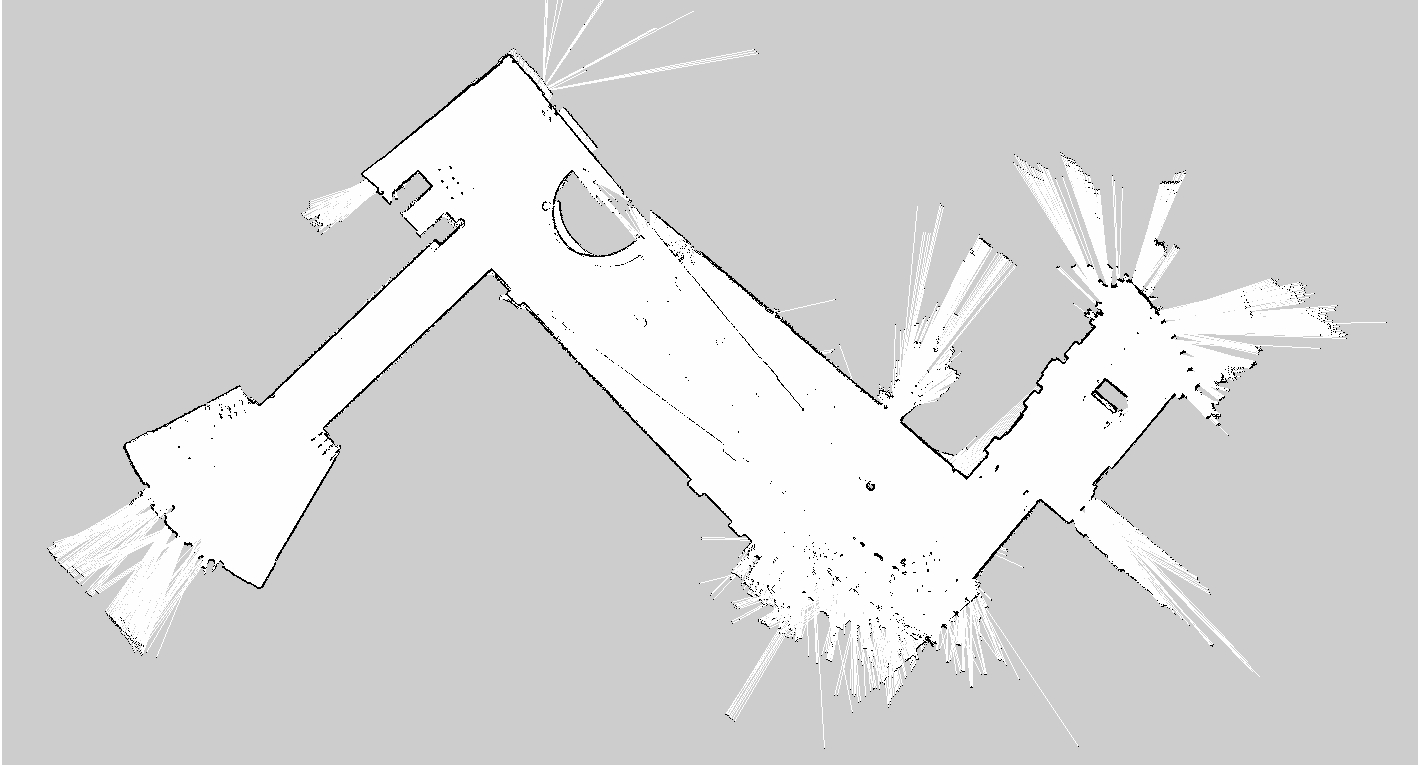
\includegraphics[width=0.5\textwidth]{pictures/firstMap.jpg}
	\caption{lol}
\end{figure}


eigene Karte einfügen. AMCL erwähnen.


\section{Pfadverfolgung mit Giovanni Indiveri}
\section{Zusammenfassung und Ausblick}


\newpage
{%\small                   % use small if you need it
	\bibliographystyle{plain}
	\bibliography{gmapping}       % use a bib-file paper.bib to collect your references
}
\end{document}



